\documentclass{classe}
\title{Ray Tracing\\ \small Cours TalENS n°1}
\author{Matthieu Boyer \& Clément Allard}
\date{16 Novembre 2024}

\usepackage[pdftex,outline]{contour}
\definecolor{v}{HTML}{00ffff}
\tikzstyle{verre} = [draw = v, fill = v!30]
\usetikzlibrary{decorations}

\newcommand{\point}[3]{\draw (#1 -.1, #2 -.1) -- (#1 + .1, #2 + .1);
\draw (#1 +.1, #2 -.1) -- (#1 - .1, #2 + .1);
\draw (#1, #2) node[below right]{#3};}

\renewcommand*{\K}{\mathbb{K}}
\graphicspath{{./Images/}}

\begin{document}
\section{Faire briller une vache de mille feux ?}
\subsection{Introduction}
\subsection{La lumière, kéazko ?}
Qu'est ce que la lumière ? Comment se propage-t-elle ? Voilà un débat qui a enflammé les derniers siècles. La conclusion de ces débats fut que la lumière se comporte comme à la fois un ensemble de photons mais également comme un onde (phénomène mis en évidence par Louis De Broglie en 1924) : on appelle ceci la dualité onde-corpuscule. Posons en premier temps la définition d'une onde :
\begin{définition}{Onde}{}
Une onde est la propagation d'une perturbation de proche en proche avec transfert d'énergie
\end{définition}
Dans le cadre du modèle de l'optique géométrique, on vient étudier le comportement de la lumière d'un point de vue simplifié, en introduisant la notion de rayon lumineux.
\begin{définition}{Rayon Lumineux}{}
On définit un rayon lumineux comme une courbe de l'espace selon laquelle se propage l'énergie lumineuse (véhiculée par l'onde).
\end{définition}
On représentera donc la lumière par des courbes fléchées.
\begin{remarque}{}{}
	D'un point de vue expérimental, la modélisation de la lumière par des rayons lumineux fonctionne bien (dans la limite d'objets assez grands devant la longueur d'onde de l'onde, pour ne pas avoir de diffraction).
\end{remarque}{}{}
\begin{figure}[H]
	\centering
	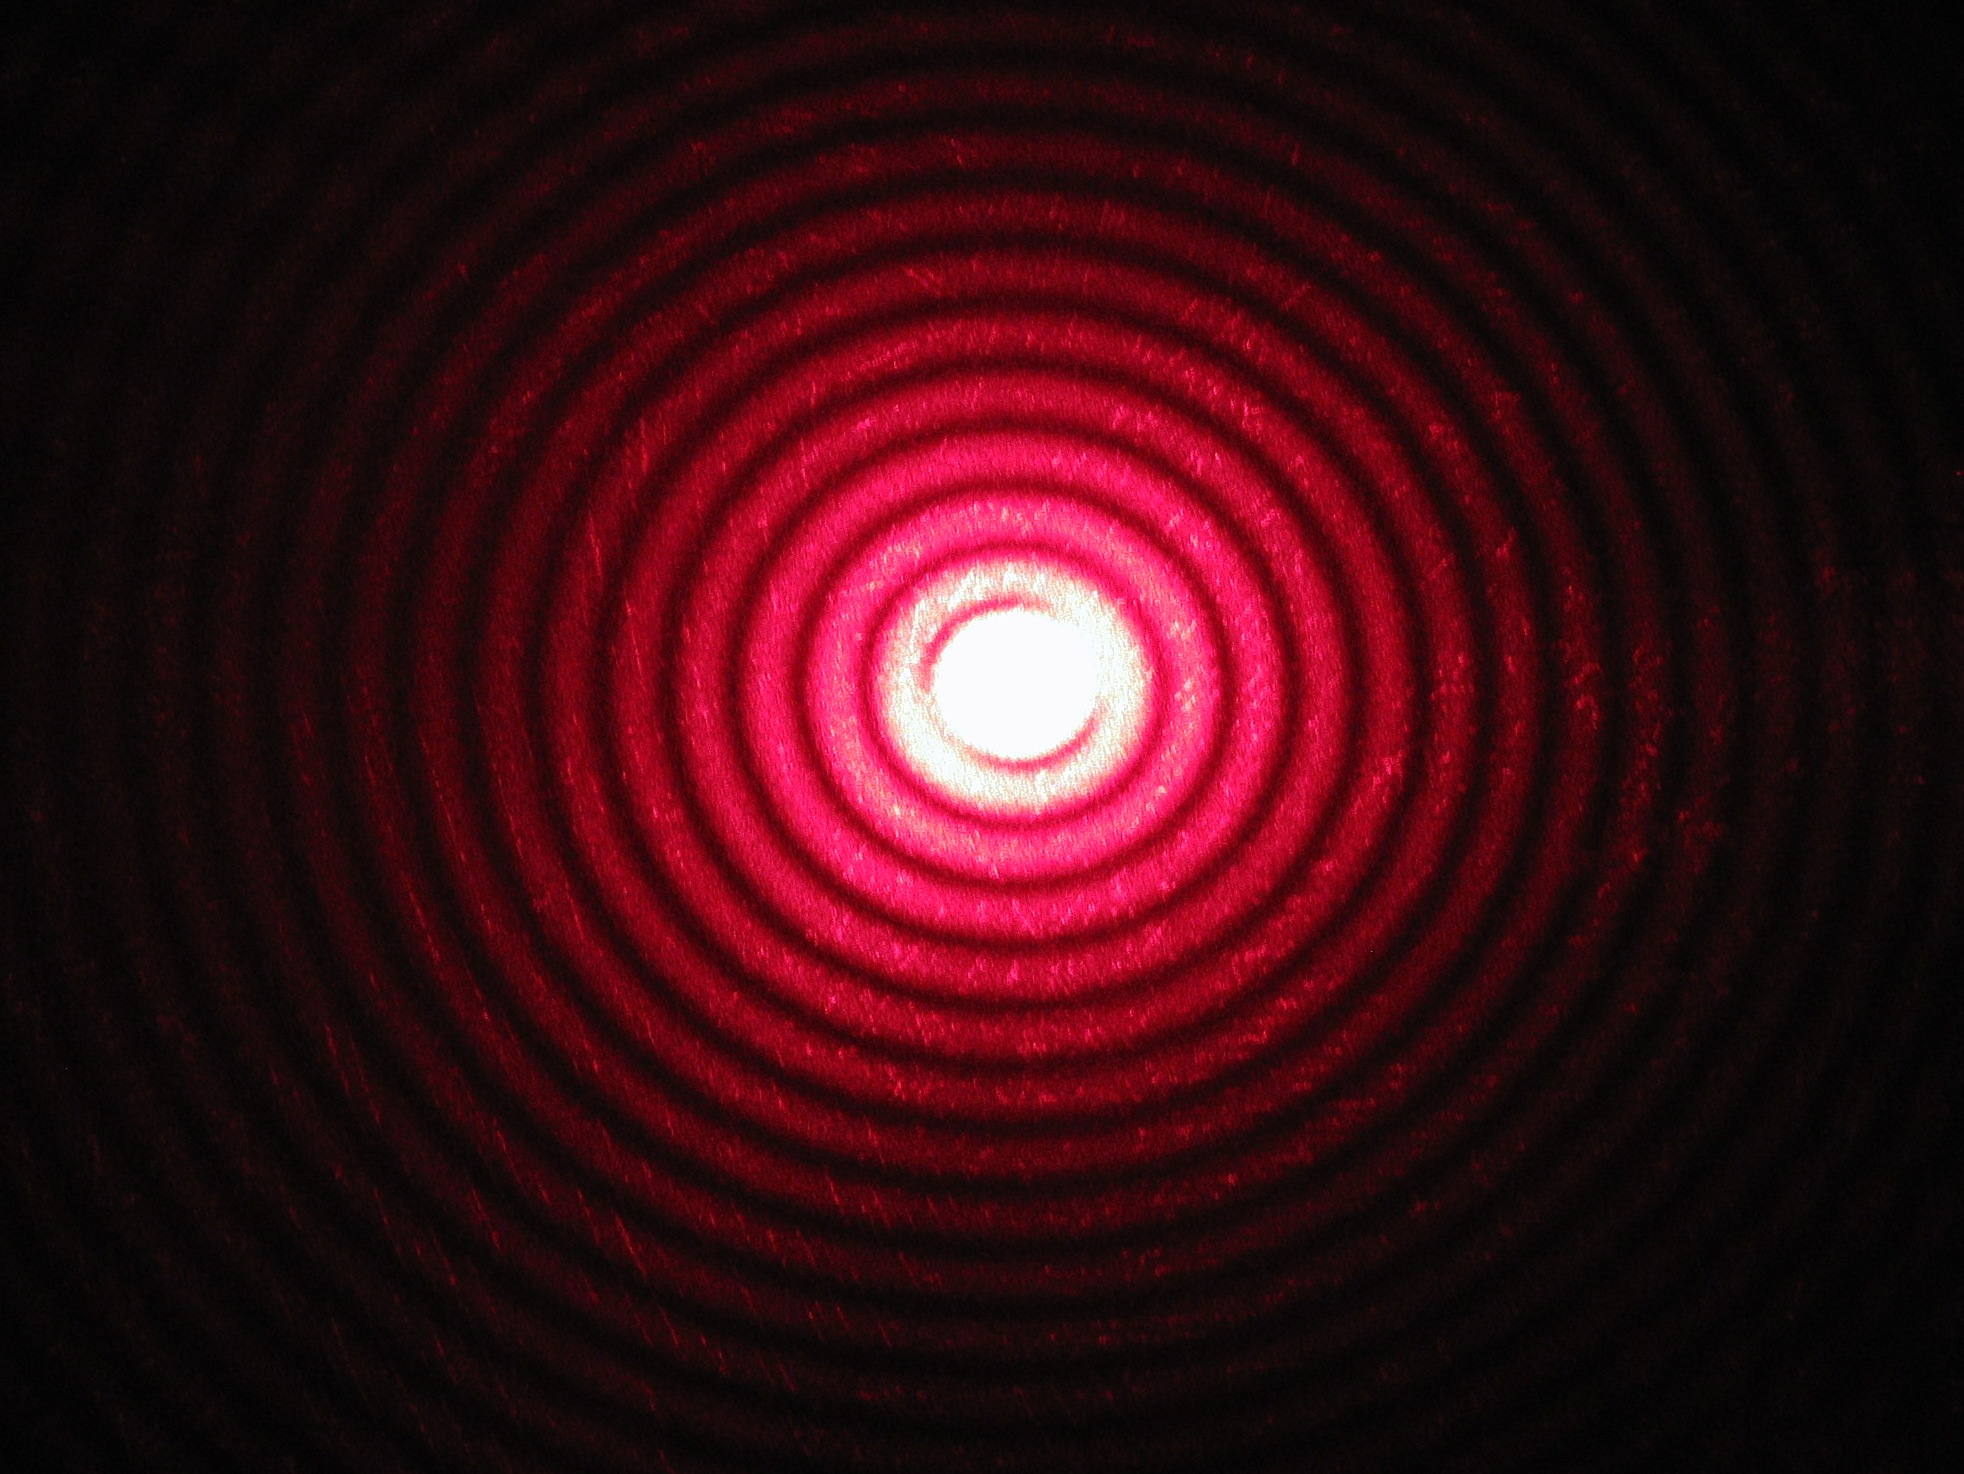
\includegraphics[scale=.08]{Diffraction.jpeg}
	\caption{Illustration du phénomène de diffraction}
\end{figure}
Nous avons à présent un modèle pour la lumière, et nous allons pouvoir étudier son devenir.

\section{Comment voit-on la vache ?}
\subsection{Propagation de la lumière}
Étudions la propagation de la lumière dans certains milieux que nous allons définir ci-dessous.
\begin{définition}{MTHI - Milieux Transparents Homogènes Isotropes}{}
On s'intéresse à des milieux qui sont :\\
- Transparents : l'énergie lumineuse n'est pas absorbée par le milieu;\\
- Homogènes : les propriétés du milieu ne dépendent pas du point choisi;\\
- Isotropes : les propriétés du milieu ne dépendent pas de la direction du rayon lumineux.
\end{définition}
\begin{définition}{Dioptre}{}
On appelle dioptre l'interface entre deux milieux
\end{définition}
Cet ensemble de milieux regroupe par exemple le vide, l'air, l'eau ou bien le verre. On peut se demander à quelle vitesse se propagent les rayons lumineux dans notre milieu, ce qui nous amène à introduire la notion d'indice optique :
\begin{définition}{Indice optique}{}
On définit l'indice optique $n$ de la manière suivante
\begin{equation*}
	n=\frac{c}{v_\varphi}
\end{equation*}
où $c =\unit{299~792~458}{\meter\cdot\second^{-1}}$ est la vitesse de la lumière dans le vide et $v_\varphi$ est la vitesse de propagation de la lumière dans notre milieu.
\end{définition}
\begin{example}
	L'indice optique du vide vaut $1$, celui de l'air $1.0003$, celui de l'eau $1.33$ et le verre autour de $1.5$.
\end{example}
\begin{théorème}{Propagation de la lumière dans les MTHI}{}
- Les rayons lumineux sont des droites;\\
- Les rayons lumineux se propagent indépendamment entre eux.
\end{théorème}
\begin{proof}
	On prouvera un de ces points ultérieurement.
\end{proof}
Un des principes fondamentaux de la propagation de la lumière dans les MTHI est le suivant :
\begin{théorème}{Principe du retour inverse de la lumière}{}
Le trajet de la lumière ne dépend pas du sens de parcours
\end{théorème}
\begin{proof}
	Ceci s'illustre car le milieu est homogène et isotrope.
\end{proof}
\subsection{Fonctionnement du ray tracing}
Considérons une lampe qui éclaire notre vache. Nous nous demandons comment un observateur extérieur peut voir la vache.


Une idée naïve serait de prendre notre source lumineuse, de déduire la marche d'un rayon lumineux (à l'aide de lois que nous verrons plus tard).
% mettre une figure pour illustrer ceci
Le problème ici est qu'on doit tracer la marche d'un grand nombre de rayons pour avoir une image de bonne résolution, sachant que la plupart des rayons n'atteindront jamais l'observateur !
% mettre une figure pour illustrer ceci
Pour nous sauver, le principe de retour inverse de la lumière vient à notre rescousse ! En effet, il suffit de tracer les rayons dirigés de l'\oe il vers la vache, et ensuite voir si le rayon intercepte notre source lumineuse.
% figure !
L'avantage : on peut se restreindre à un nombre de rayons plus limité, en ne prenant que ceux qui vont entrer dans le champ de vision de l'observateur et économisant énormément de puissance de calcul (ce qui est nécessaire pour la fluidité d'un jeu vidéo).

\section{Implémentation pratique}
\subsection{Comment prédire la trajectoire de la lumière ?}
Une règle fondamentale permet de prédire la trajectoire de la lumière :
\begin{théorème}{Principe de Fermat}{}
La lumière se propage en minimisant son temps de parcours.
\end{théorème}
\begin{remarque}{}{}
Ce principe n'est pas exclusif à la lumière, et par exemple est aussi vrai pour le son (et généralement tout comportement ondulatoire) : on peut donc faire des équivalents de ray tracing sur du son ou autres.
\end{remarque}{}{}
En notant une distance $AB$, on a :
\begin{equation*}
	\Delta t = \frac{AB}{v_\varphi} = \frac{nAB}{c}
\end{equation*}
On note $(AB) = nAB$ le chemin optique. Le principe de Fermat s'écrit de manière équivalente en la minimisation du chemin optique.\\
\begin{remarque}{}{}
	Dans un milieu d'indice constant, la minimisation du chemin optique est équivalente à celle de la distance entre deux points. On sait que le chemin le plus court entre deux points est la ligne droite : on retrouve que dans un MTHI, les rayons lumineux sont des droites.
\end{remarque}
Ce principe permet d'intuiter les lois dites de Snell-Descartes :
\begin{théorème}{Lois de Snell-Descartes}{}
À l'interface entre deux milieux d'indice optique $n_1$ et $n_2$, la propagation d'un rayon lumineux en provenance du milieu $1$ se fait selon les lois suivantes :
\begin{itemize}
	\item\color{vulm}{Plan d'incidence :}\ \color{black} Il existe un rayon réfléchi (qui reste dans le milieu $1$) et un rayon réfracté (qui se propage dans le milieu $2$) qui sont tous les deux situés dans le plan formé par le rayon incident et la normale au dioptre.
	\item \color{vulm}{Réfraction :}\ \color{black} L'angle $i_{2}$ de sortie dans le milieu $2$ vérifie \[n_{1}\sin{\left(i_{1}\right)} = n_{2}\sin{\left(i_{2}\right)}\]
    \item \color{vulm}{Réflexion :}\ \color{black} Son angle $i_{1}'$ de réflexion dans le milieu $1$ est tel que la normale au milieu au point d'incidence est la bissectrice de l'angle $i_{1} + i_{1}'$.
\end{itemize}
\end{théorème}
\begin{tabular}{m{.3\linewidth}m{.6\linewidth}}
    Loi de la Réfraction :
    \[
        n_{1}\sin{\left(i_{1}\right)} = n_{2}\sin{\left(i_{2}\right)}
    \]
     &
    \begin{tikzpicture}[scale=1.25,x={(-0.353cm,-0.353cm)}, y={(1cm,0cm)}, z={(0cm,1cm)},>=stealth]
        \coordinate (O) at (0, 0, 0);
        \coordinate (A) at (2,2,0);
        \coordinate (M) at (3,4,0);
        \coordinate (B) at (2,2,-2);
        \draw[verre] (O) -- ++(4, 0, 0) ;
        \draw[verre] (O) -- +(0, 4, 0) ;
        \draw[verre](O) --++(4,0,0)--++(0,4,0)--++(-4,0,0)--cycle;
        \draw[verre](0,4,0) --++(0,0,-2)--++(4,0,0)--++(0,0,2)--cycle;
        \draw[verre](4,0,0) --++(0,0,-2)--++(0,4,0)--++(0,0,2)--cycle;
        \draw[vulm](4,2,-2)--++(0,0,4)--++(-4,0,0)--++(0,0,-4)--cycle;
        \draw[vulm] (4,2,-2) node[rotate=45,below right]{\small \hspace{10pt}Plan d'Incidence};
        \draw[dashed, vulm] (A) ++(2,0,0)--++(-4, 0, 0) ;
        \draw[->,thick,postaction={decorate},red] (4,2,1.5)--(A);
        \draw[->,thick,postaction={decorate},red] (A)--(0.4,2,-2);
        \draw[dashed, vulm, ->] (B)--++(0,0,4.5)node[below left, fill = none]{\small Normale};%la normale
        \draw[vulm] (2,2,0.5) to[bend right, vulm] (2.65,2,0.5);
        \draw (2.55,2,0.8) node[vulm]{$i_{1}$};
        \draw[vulm] (2,2,-0.5) to[bend right, vulm] (1.5,2,-0.6);
        \draw (1.55,2,-0.8) node[vulm]{$i_{2}$};
        \draw (2,0,1) node[vulm]{Indice $n_{1}$};
        \draw (2,0,-2) node[vulm]{Indice $n_{2}$};
    \end{tikzpicture}
\end{tabular}

\begin{tabular}{m{.3\linewidth}m{.6\linewidth}}
    Loi de la Réflexion:
    \[
        i_{1} = -i_{1}'
    \]
     &
    \begin{tikzpicture}[scale=1.25,x={(-0.353cm,-0.353cm)}, y={(1cm,0cm)}, z={(0cm,1cm)},>=stealth]
        \coordinate (O) at (0, 0, 0);
        \coordinate (A) at (2,2,0);
        \coordinate (M) at (3,4,0);
        \coordinate (B) at (2,2,-2);
        \draw[verre] (O) -- ++(4, 0, 0) ;
        \draw[verre] (O) -- +(0, 4, 0) ;
        \draw[verre](O) --++(4,0,0)--++(0,4,0)--++(-4,0,0)--cycle;
        \draw[verre](0,4,0) --++(0,0,-0.5)--++(4,0,0)--++(0,0,0.5)--cycle;
        \draw[verre](4,0,0) --++(0,0,-0.5)--++(0,4,0)--++(0,0,0.5)--cycle;
        \draw[vulm](4,2,-2)--++(0,0,4)--++(-4,0,0)--++(0,0,-4)--cycle;
        \draw[vulm] (4,2,-2) node[rotate=45,below right]{\small Plan d'Incidence};
        \draw[dashed, vulm] (A) ++(2,0,0)--++(-4, 0, 0) ;
        \draw[->,thick,postaction={decorate},red] (4,2,1.5)--(A);
        \draw[->,thick,postaction={decorate},red] (A)--(0,2,1.5);
        \draw[dashed, vulm, ->] (B)--++(0,0,4.5)node[above,fill=none]{\small Normale\hspace{12pt}};%la normale
        \draw[vulm] (2,2,0.5) to[bend right] (2.65,2,0.5);
        \draw (2.55,2,0.8) node[vulm]{$i_{1}$};
        \draw[vulm] (2,2,0.75) to[bend left] (1.25,2,0.6);
        \draw (1.55,2,0.9) node[vulm]{$i'_{1}$};
        \draw (2,0,1) node[vulm]{Indice $n_{1}$};
        \draw (2,0,-1) node[vulm]{Indice $n_{2}$};
    \end{tikzpicture}
\end{tabular}

\begin{proof}
\begin{itemize}
	\item \color{vulm}{Plan d'incidence :}\ \color{black} Soient deux points dans le plan d'incidence. Pour le cas de la réfraction, le rayon de Snell-Descartes minimise la durée de parcours totale comparé à un rayon qui ne serait pas dans le plan d'incidence. Pour la réflexion, c'est la même chose sauf qu'on a comme contrainte que le rayon passe par le dioptre.
	\item \color{vulm}{Réflexion :}\ \color{black} On sait que nos rayons sont dans le plan d'incidence. On doit minimiser la distance entre deux points $A$ et $B$ avec comme condition le fait qu'on passe par le dioptre :
	\begin{figure}[H]
	\centering
	\begin{tikzpicture}
		\draw[vulm] (-2, -2) -- (-2, 2) -- (2, 2) -- (2, -2) -- cycle;
		\draw (0, 2) node[above]{Plan d'incidence};
		\point{-1}{1}{$A$};
		\point{1}{1.5}{$B$};
		\point{-.4}{0}{$D$};
		\draw[->] (0, .2) -- (-.4, .2);
		\draw (-.2, .2) node[above]{$x$};
		\draw[->] (-1, 0)  -- (-1, 1);
		\draw (-1, .5) node[left]{$d_1$};
		\draw[->] (1, 0)  -- (1, 1.5);
		\draw (1, .75) node[right]{$d_2$};
		\draw[->, red, thick] (-1, 1) -- (-.7, .5);
		\draw[->, red, thick] (-.7, .5) -- (-.4, 0);
		\draw[->, red, thick] (-.4, 0) -- (0.3, .75) -- (1, 1.5);
		\draw[->, red, thick] (0.3, .75) -- (1, 1.5);
		\draw[<->] (-1, -.5) -- (0, -.5);
		\draw (-.5, -.5) node[below]{$d_3$};
		\draw[<->] (1, -.5) -- (0, -.5);
		\draw (.5, -.5) node[below]{$d_4$};
		\draw[dashed, vulm] (-2.5, 0) -- (2.5, 0);
		\draw[dashed, vulm] (0, -2.5) -- (0, 2.5);
	\end{tikzpicture}
	\end{figure}
	\noindent On doit donc minimiser (étant donné que l'indice optique est constant, minimiser le temps revient à minimiser la distance)
	\begin{equation*}
	d(x) = \sqrt{d_1^2+(d_3+x)^2} + \sqrt{d_2^2+(d_4-x)^2}
	\end{equation*}
	En dérivant et cherchant les extrema (on annule la dérivée), on trouve que $i_1$ = $i'_1$
	\item \color{vulm}{Réfraction :}\ \color{black} Principe analogue à la réflexion.
	
\end{itemize}
\end{proof}
Nous avons à présent un moyen de prédire la trajectoire des rayons lumineux à l'aide de la connaissance des indices optiques.

\end{document}
